\section{Experimental Procedure}
\label{sec:ExpProc}
Nine CBC3 chips were irradiated, using the CERN Seifert RP149 X-ray machine, at a variety of dose rates (${0.11\pm0.02}$\kGyH to ${23.0\pm4.6}$\kGyH) and temperatures (${-20}$\deg to ${5}$\deg). The temperature of the chips were controlled and monitored throughout the irradiation, and the dose rates were measured, with an uncertainty of ${20}$\%, using a calibrated PIN diode. 
%machine's high-power cooling system was used to control the temperature of the chips, monitored using a thermocouple placed close to the chip, during irradiation. 
%connected to a source-measure unit with a high-precision ammeter.
%and its dry-air injection system was used to prevent condensation.
% Is the temperature statement true or necessary? The dew point in Geneva is often close to 20C.
% S.S changed 
%A thermocouple, placed close to the chip, was used to measure the temperature inside the X-ray chamber. 
% S.S - removed the table and added a line to the test indicating the dose rates used 
% \Cref{tab:calibration} summarizes the X-ray tube settings and  dose rates used for the CBC3 irradiation campaign.
% The voltage applied to the diode is 50~V and the actual dose rate is then computed from the measured current using the calibration \cref{eq:doserate}. 
% \begin{equation}
%     \dot{D}\,[\text{kGy}/\text{h}]=1.3728\times10^{-7}~\times~I\,[\text{A}]
%     \label{eq:doserate}
% \end{equation}
% \begin{figure}[!htbp]
% \centering
% 	% Is this table really necessary? All the reader cares about is the dose rates,
%     % so could say above "at dose rates from X to Y."
%     % Also should not be part of a figure, it's a table.
% 	\subfloat[Dose rates table][X-ray tube settings used for the CBC3 X-ray irradiation. 
%     %The dose was changed by adjusting either the vertical position of the CBC3 w.r.t the tube or by changing the tube's supply current.
%     ]
%   {
%     \begin{tabular}{cccc}
%     \midrule
%         Voltage & Current & Distance & Dose Rate\\
%         $[$kV$]$ & $[$mA$]$ & $[$cm$]$ & $[$\kGyH$]$\\
%     \midrule
%     %\hline
%     $50$ & $40$ & $8$  & ${23.0\pm4.6}$\\
%     $50$ & $20$ & $8$  & ${11.6\pm2.3}$\\
%     $50$ & $10$ & $8$  & ${5.8\pm1.2}$\\
%     $50$ & $13$ & $18$ & ${2.4\pm0.5}$\\
%     $50$ & $10$ & $32$ & ${0.11\pm0.02}$\\
%     \midrule 
%   	\end{tabular}
%     \label{tab:calibration}
%   }
%   \quad
%   \subfloat[DAQ schematic][Schematic of the data acquisition and monitoring system used in the radiation tests.]
%   {
% % I'd be tempted to drop this if space requires (plus the reference in the text of course)
% 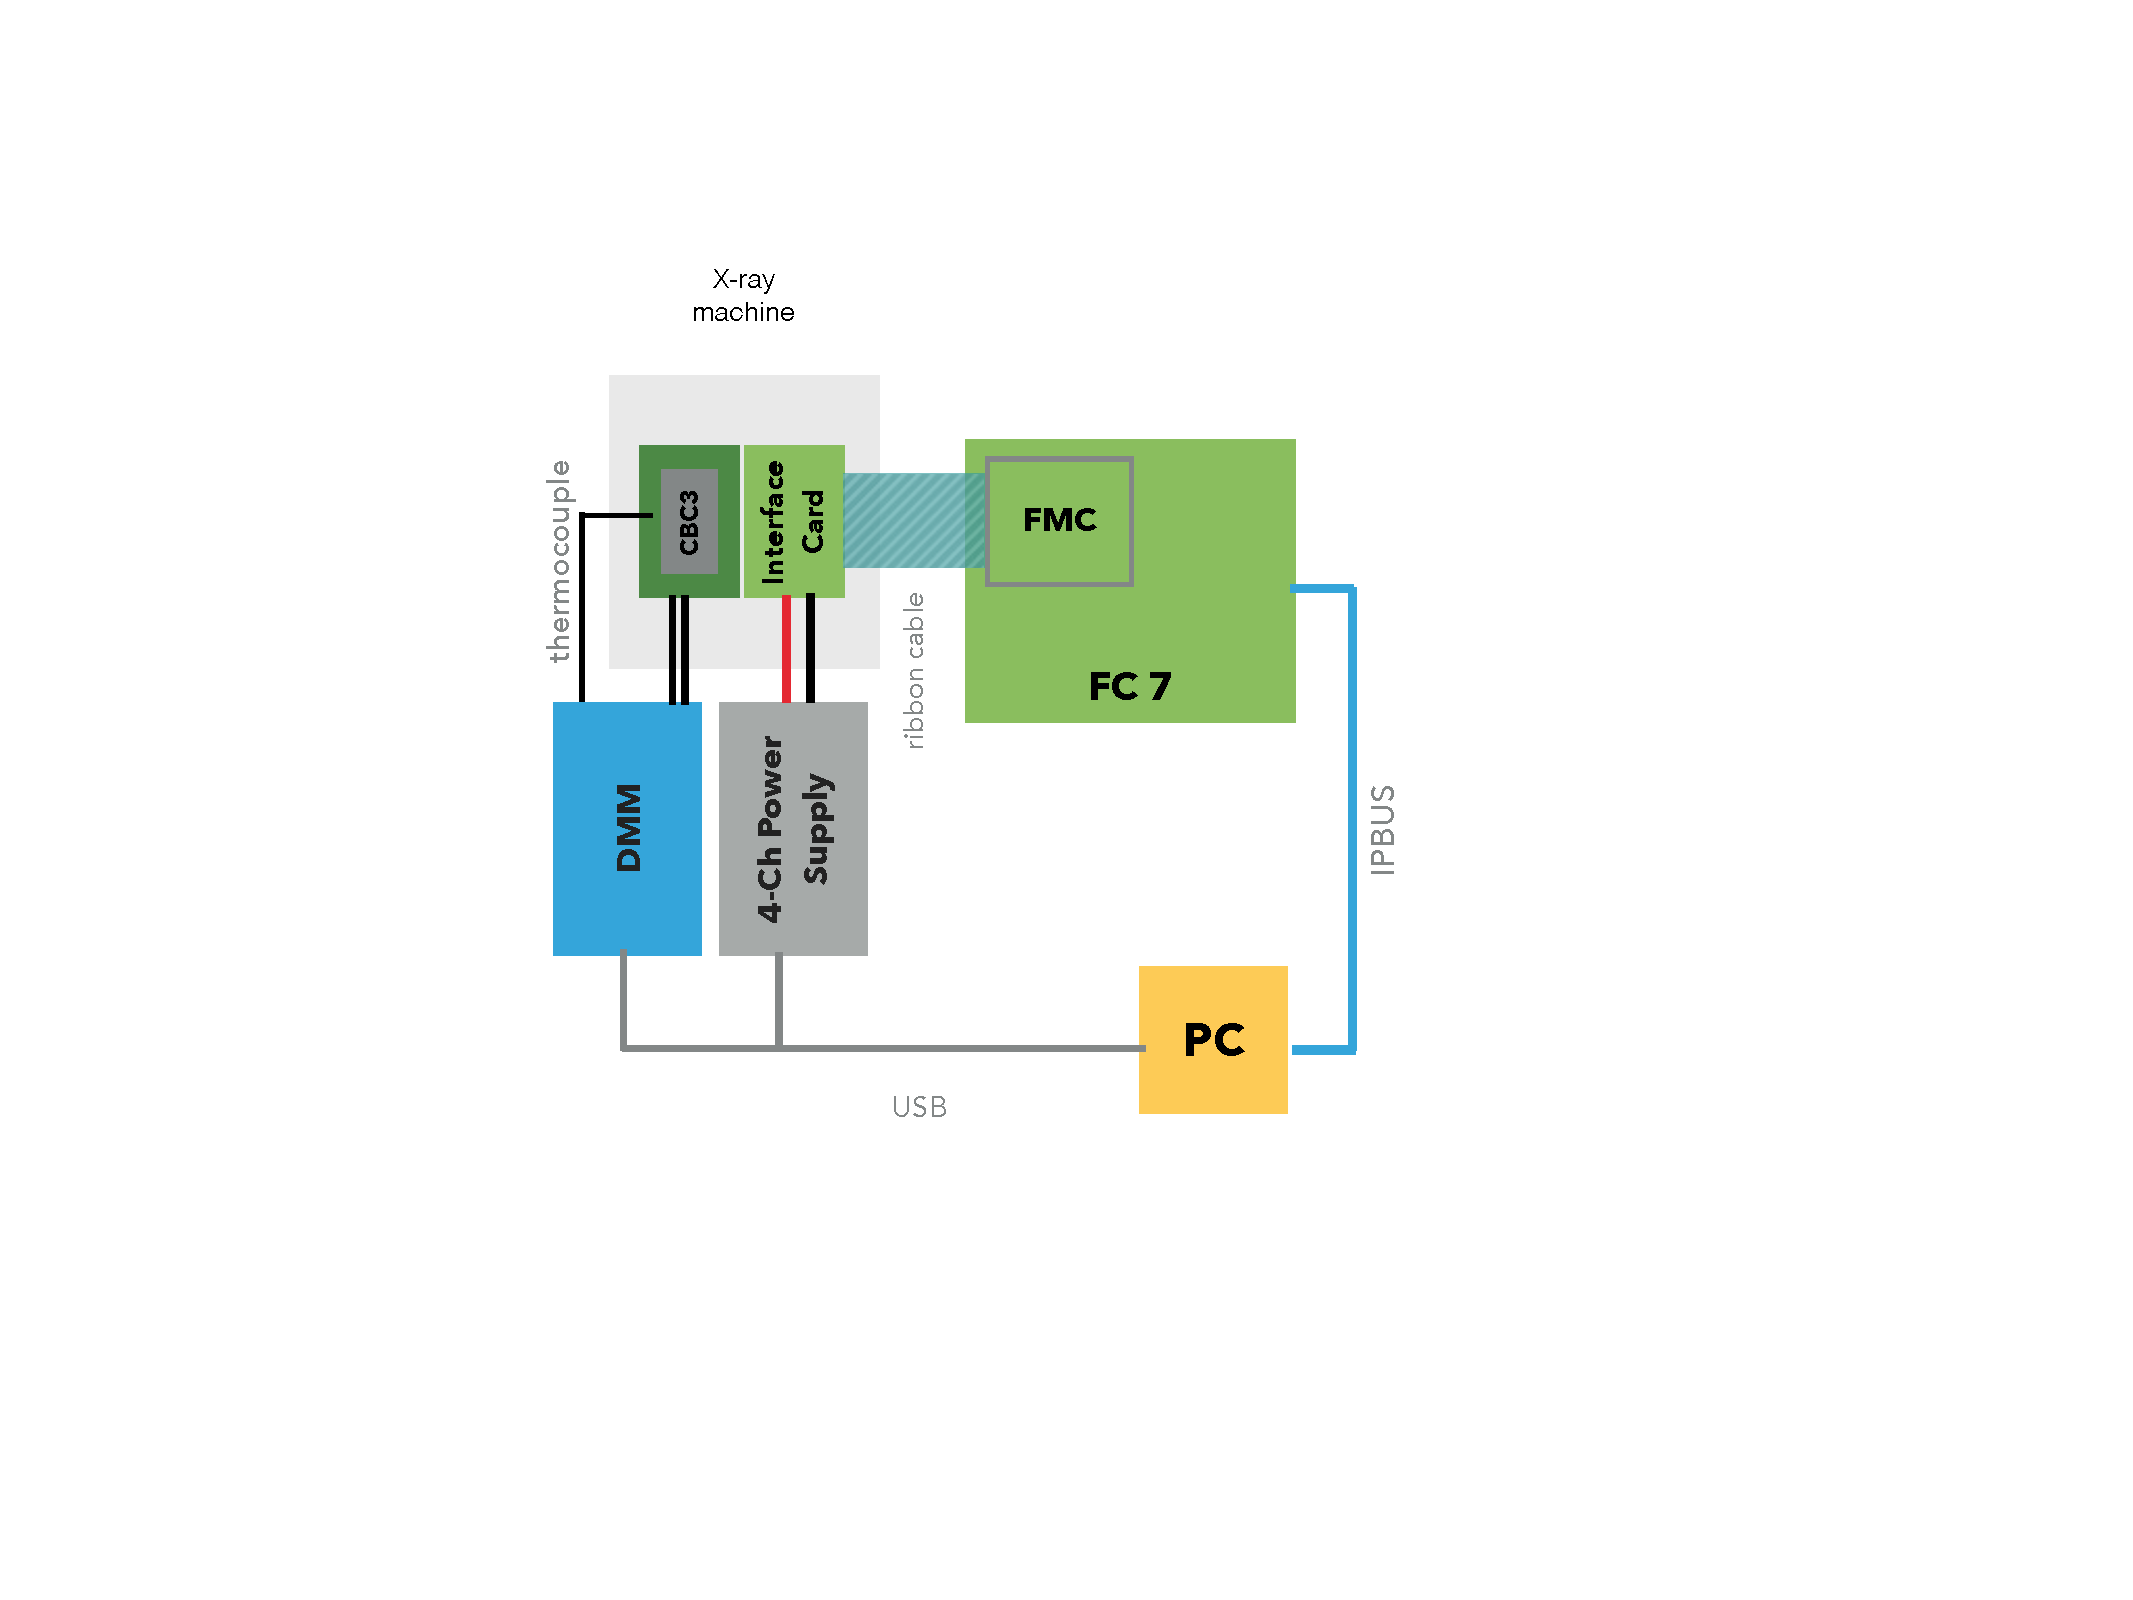
\includegraphics[width=0.8\linewidth]{Figures/SchematicSetup.pdf}
%   	\label{fig:daq}
%   }
%   \caption[Fit.]{DAQ system consisting of an FC7, a \textmu TCA Advanced Telecommunications Computing Architecture (ATCA) card and an interface card. A 1.5~m shielded ribbon cable was used to connect the interface card to the FC7 via a custom FPGA Mezanine Card.}
%   \label{fig:tst}
% \end{figure} 

% \begin{table}[htbp!]
% \begin{center}
%     \begin{tabular}{cccc}
%     \midrule
%         Voltage & Current & Distance & Dose Rate\\
%         $[$kV$]$ & $[$mA$]$ & $[$cm$]$ & $[$\kGyH$]$\\
%     \midrule
%     %\hline
%     $50$ & $40$ & $8$  & ${23.0\pm4.6}$\\
%     $50$ & $20$ & $8$  & ${11.6\pm2.3}$\\
%     $50$ & $10$ & $8$  & ${5.8\pm1.2}$\\
%     $50$ & $13$ & $18$ & ${2.4\pm0.5}$\\
%     $50$ & $10$ & $32$ & ${0.11\pm0.02}$\\
%     \midrule 
%   	\end{tabular}
% \caption{Dose rates and settings used for the CBC3 X-ray irradiation. The uncertainty on the dose rate is assumed to be 20\% of the value measured with the calibrated PIN diode. The dose was changed by adjusting either the vertical position of the CBC3 wrt the tube or by changing the tube's supply current.}
% \label{tab:calibration}
% \end{center}
% \end{table}
% don't really have space for this 
% \begin{figure}[htbp]
% \centering
% 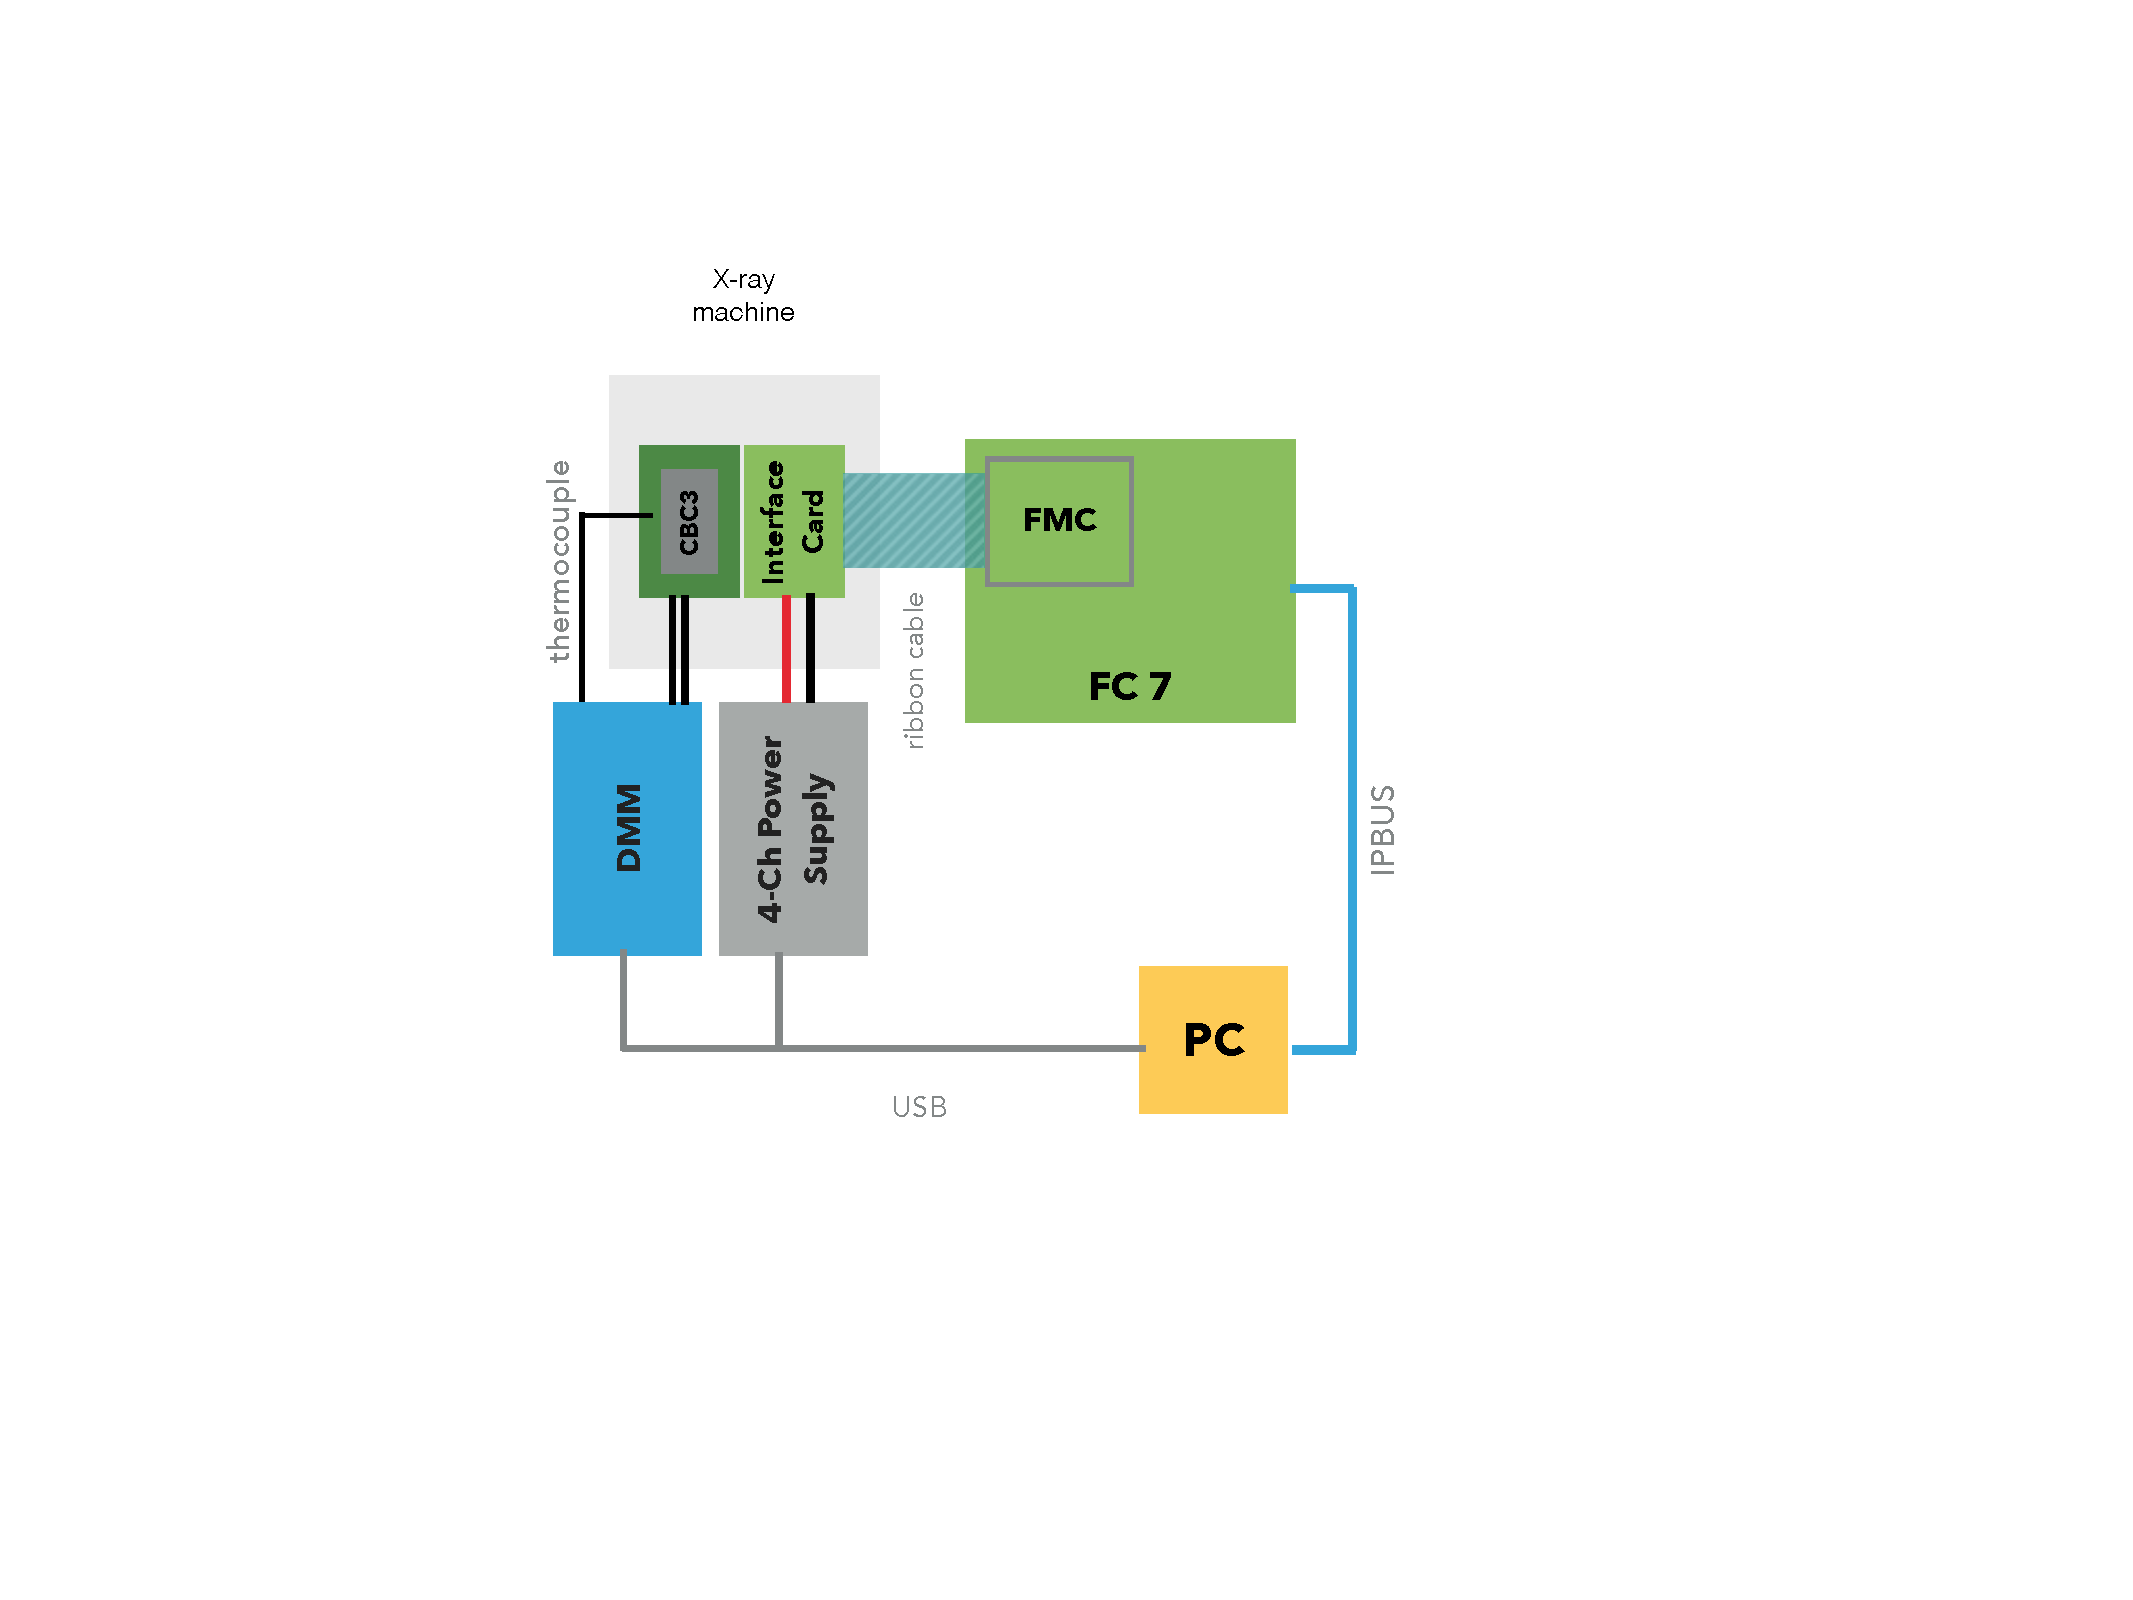
\includegraphics[width=0.65\linewidth]{Figures/SchematicSetup.pdf}
% \caption{DAQ system consisting of an FC7, a \textmu TCA Advanced Telecommunications Computing Architecture (ATCA) card and an interface card. A 1.5~m shielded ribbon cable was used to connect the interface card to the FC7 via a custom FPGA Mezanine Card.}
% \label{fig:daq}
% \end{figure}

To replicate realistic operating conditions, a prototype DAQ system  was used to provide the 320~MHz system clock, slow-control I2C commands, and clock-synchronous fast commands such as triggers and resets. The chips were wire-bonded to carrier boards plugged into an interface card, which provided the low voltage (1.25V) and level translation to interface to the DAQ. The interface card also provided monitoring of the digital and analogue currents, and the on-chip analogue bias signals.
% (via an on-chip 17:1 analogue multiplexer).

% A standard measurement cycle was repeated throughout the irradiation. The CBC3 was reconfigured at the start of each cycle. A tuning algorithm, designed to offset The individual channel offsets were then adjusted for a uniform response across the whole chip, with and without a test-pulse injected. This ensures that the global threshold is the same for all input channels and allows the measurement of the pedestal (the threshold corresponding to a noise occupancy of 50\%) and the noise per input channel. After calibration, the chip is triggered for a period of ten minutes at a high trigger rate with a channel occupancy of around 50\%, to ensure a high level of digital activity. The final part of the cycle involves stepping each analogue bias DAC setting through its full range, while holding the other DAC settings at their nominal values. The analogue biases are monitored externally with the multimeter, so this confirms the actual voltage for each DAC setting and checks if any of the control registers change their behavior in response to ionizing radiation. 